\documentclass[11pt, a4paper]{article}

\usepackage{style}

\author{Vladislav Mlejnecký}

\title{%
  Číslicové zpracování signálů\\
  \large Úloha číslo 3.\\
  Vzorkovací kmitočet, aliasing a kvantizace signálů v amplitudě}

\begin{document}

    \maketitle

    \section{Zadání}
    
    Do lokálního počítače si stáhněte soubory Ukaz1.wav a Ukaz2.wav ze Stagu. Oba soubory jsou ve formátu mono, 16 bitů, vzorkování 44100Hz.

    \begin{enumerate}
        \item
        V jazyku Matlabu napište kód, kterým načtete soubor Ukaz1 do paměti a přehrajte jej 
        \begin{enumerate}[label=(\alph*)]
            \item
            nejprve v původním formátu, 
            \item
            po té se vzorkovací frekvencí 8.82 kHz, 
            \item
            následně se vzorkovací frekvencí 4.41 kHz. 
        \end{enumerate}
        
        Totéž proveďte pro druhý soubor Ukaz2.wav. Všechny ukázky přehrajte v jednom m-souboru. Poslechněte a popište pozorovaný jev. Zejména ve zvuku c) oproti a) něco chybí a něco přebývá.
        
        \item
        
        V jazyku Matlabu napište kód, kterým načtete soubor Ukaz1 do paměti a přehrajte jej 
        
        \begin{enumerate}[label=(\alph*)]
            \item
            nejprve v původním formátu, 
            \item
            po té  s kvantizací 6 bitů, 
            \item
            následně se vzorky o velikosti 4 bity.
            \item
            oba případy b) a c) znázorněte zobrazením v grafu, zobrazte asi 10000 vzorků
        \end{enumerate}
        Totéž proveďte v témže m-souboru i pro druhý zvukový soubor Ukaz2.wav. Poslechněte a popište pozorovaný jev. Podobně jako v bodě 2. ve zvuku c) oproti a) občas něco chybí a něco přebývá, tentokrát něco jiného.
    \end{enumerate}
    
    \section{Výsledné grafy}
    
        \begin{figure}[H]
            \centering
            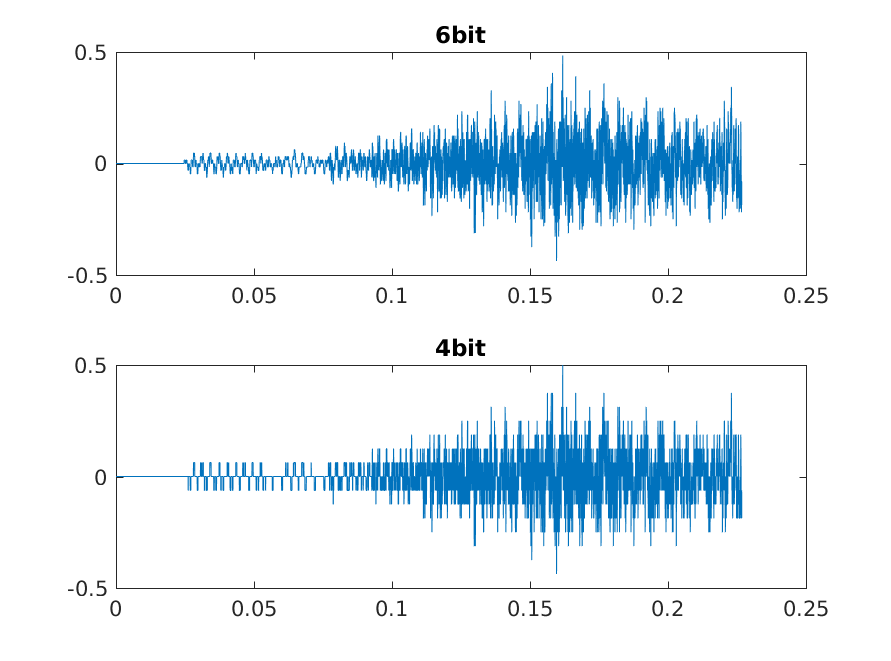
\includegraphics[width=.7\textwidth]{matlab/Ukaz1.png}
            \caption{Změna rozlišení pro ukázku 1}
            \label{fig:graf1}
        \end{figure}
        
        \begin{figure}[H]
            \centering
            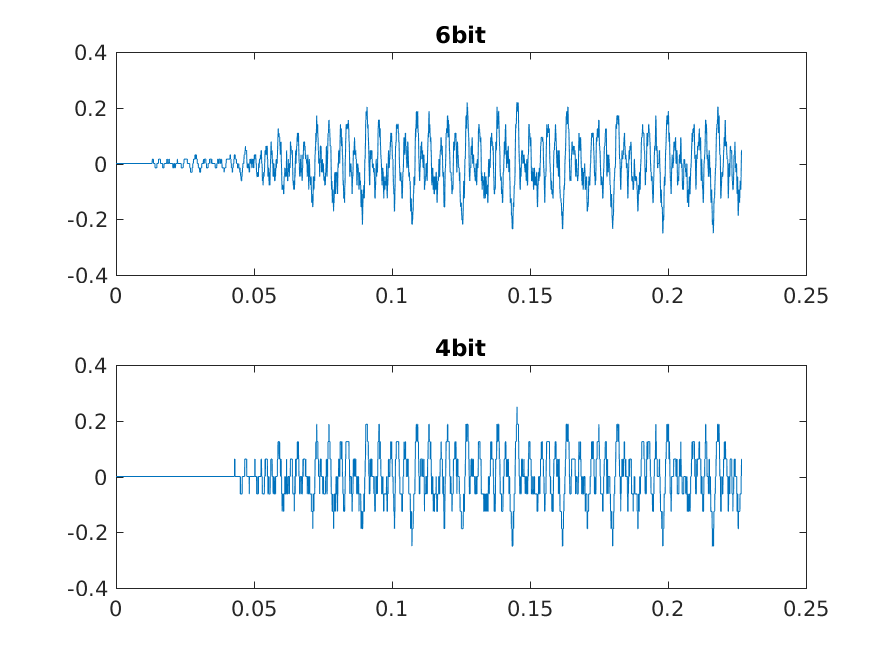
\includegraphics[width=.7\textwidth]{matlab/Ukaz2.png}
            \caption{Změna rozlišení pro ukázku 2}
            \label{fig:graf2}
        \end{figure}
        
    \section{Komentář k výsledkům}
        
        V prvním bodě zadání se s klesající vzorkovací frekvencí 
        snižuje kvalita audio záznamu. Dochází totiž k jevu zvanému 
        aliasing který je způsoben nedostatečnou vzorkovací frekvencí. 
        Snižování vzorkovací frekvence je zde suplováno decimací. Pro 
        decimaci nelze použít funkci již v Matlabu obsaženou, protože 
        ta před decimací aplikuje na vstupní posloupnost lowpass filtr.
        
        Snížením vzorkovací frekvence snížíme maximální možnou 
        frekvenci která se může v digitálním signálu vyskytovat dle 
        Shannonova vzorkovacího teorému. My toto ovšem porušujeme 
        protože v původním signálu jsou obsaženy i vyšší frekvence, 
        výsledný zvuk je tedy zkreslený. Zároveň dochází k překlopení 
        části spektra nad polovinou vzorkovací frekvence zpět, což 
        kvalitu ještě více snižuje.
        
        Rozdíl v kvalitě je lépe slyšet na první ukázce neboť ta má 
        mnohem širší spektrum nežli ukázka druhá.
        
        V druhém bodě se snižuje rozlišení vzorkování vstupních dat. 
        Tím se samozřejmě opět snižuje kvalita audio záznamu, tentokrát 
        ovšem díky jevu známému jako kvantizační šum. Vstupní hodnota 
        je totiž při diskretizaci v amplitudě zaokrouhlena na nejbližší 
        kvantizační úroveň.
        
        Při rozlišení 6 bitů jsem nebyl schopen zaznamenat výrazné 
        zhoršení kvality, ovšem při použití bitů čtyř je již slyšet 
        výrazný šup na pozadí skladby.
        
    \section{Výpis zdrojového kódu}
    
\begin{lstlisting}[language=matlab, frame=single]    
mute = 0;
ukol1('Ukaz1.wav', mute);
ukol1('Ukaz2.wav', mute);
ukol2('Ukaz1.wav', mute);
ukol2('Ukaz2.wav', mute);

function ukol2(fileName, mute)
    
    disp(['File ' fileName]);
    
    [ukazka_orig, Fs] = audioread(fileName);
    
    disp('playing original');
    playerobj = audioplayer(ukazka_orig, Fs);    
    play_muteable(playerobj, mute);

    audio_6 = change_resolution(ukazka_orig, 6);
    disp('playing 6bit');
    playerobj = audioplayer(audio_6, Fs);
    play_muteable(playerobj, mute);

    audio_4 = change_resolution(ukazka_orig, 4);
    disp('playing 4bit');
    playerobj = audioplayer(audio_4, Fs);
    play_muteable(playerobj, mute);

    h = figure();
    subplot(2, 1, 1);
    plot((0:9999)*1/Fs, audio_6(1:10000));
    title('6bit');
    subplot(2, 1, 2);
    plot((0:9999)*1/Fs, audio_4(1:10000));
    title('4bit');
    saveas(h, strrep(fileName, '.wav', '.png'));
end

function ukol1(fileName, mute)
    
    disp(['File ' fileName]);
    
    [ukazka_orig, Fs_orig] = audioread(fileName);

    for factor = [1, 5, 10]
        disp(['playing Fs = Fs_orig/' int2str(factor)])
        audio = my_decimate(ukazka_orig, factor);
        playerobj = audioplayer(audio, Fs_orig / factor);
        play_muteable(playerobj, mute);
    end
end

function out = change_resolution(x, bits)
    koef = (2^(bits))/max(abs(x));
    out = (round(x * koef))/koef;
end
    
function audio = my_decimate(x, factor)
    n = 1:factor:length(x);
    audio = x(n);
end

function play_muteable(obj, mute)
    if mute == 0
        playblocking(obj);
    end
end
\end{lstlisting}
    

\end{document}
